\subsection{How Much Motion and in Which Direction?}

The coordinate pair of a vector records two changes, but it does not immediately
answer two basic geometric questions.

\begin{corebox}[Two questions carried by every nonzero vector]
\begin{enumerate}
    \item How long is the displacement?
    \item In which direction does it point?
\end{enumerate}
\end{corebox}

Let
\[
\mathbf v=(v_1,v_2)
\]
be drawn from the origin. Its endpoint, together with its horizontal and
vertical coordinate changes, forms a right triangle. The legs have lengths
$|v_1|$ and $|v_2|$, while the vector itself is the hypotenuse.

\begin{center}
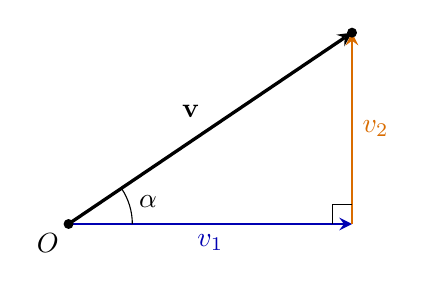
\begin{tikzpicture}[scale=0.9,>=stealth]
    \coordinate (O) at (0,0);
    \coordinate (P) at (4,2.7);
    \coordinate (R) at (4,0);

    \draw[very thick,->] (O) -- (P)
        node[midway,above left] {$\mathbf v$};
    \draw[blue!70!black,line width=1pt,->] (O) -- (R)
        node[midway,below] {$v_1$};
    \draw[orange!85!black,line width=1pt,->] (R) -- (P)
        node[midway,right] {$v_2$};
    \draw (R) ++(-0.28,0) -- ++(0,0.28) -- ++(0.28,0);

    \draw (0.9,0) arc[start angle=0,end angle=34.0,radius=0.9];
    \node at (1.12,0.32) {$\alpha$};
    \fill (O) circle (2pt) node[below left] {$O$};
    \fill (P) circle (2pt);
\end{tikzpicture}
\end{center}

\begin{derivationbox}[Length from the Pythagorean theorem]
The right triangle gives
\[
\|\mathbf v\|^2=v_1^2+v_2^2.
\]
The length is nonnegative, so
\[
\|\mathbf v\|=\sqrt{v_1^2+v_2^2}.
\]
\end{derivationbox}

\begin{definitionbox}
The Euclidean length, or norm, of $\mathbf v=(v_1,v_2)$ is
\[
\boxed{\|\mathbf v\|=\sqrt{v_1^2+v_2^2}}.
\]
The double bars distinguish the vector from the number measuring its length.
\end{definitionbox}

\begin{theorembox}
\[
\boxed{\|\mathbf0\|=0},
\qquad
\boxed{\mathbf v\neq\mathbf0\implies\|\mathbf v\|>0}.
\]
Moreover, for points $A$ and $B$,
\[
\boxed{d_E(A,B)=\|B-A\|}.
\]
\end{theorembox}

\begin{interpretationbox}[A displacement packages distance and direction]
The vector $B-A$ records how to move from $A$ to $B$, while its norm records the
Euclidean distance travelled. The same object therefore carries both directional
and metric information.
\end{interpretationbox}

Now assume $\mathbf v\neq\mathbf0$ and let $\alpha$ be its angle of inclination,
measured from the positive $x$-axis.

\begin{derivationbox}[Separating magnitude from direction]
The right triangle gives
\[
\cos\alpha=\frac{v_1}{\|\mathbf v\|},
\qquad
\sin\alpha=\frac{v_2}{\|\mathbf v\|}.
\]
Therefore
\[
v_1=\|\mathbf v\|\cos\alpha,
\qquad
v_2=\|\mathbf v\|\sin\alpha.
\]
\end{derivationbox}

\begin{theorembox}
Every nonzero vector admits the decomposition
\[
\boxed{
\mathbf v=\|\mathbf v\|(\cos\alpha,\sin\alpha)
}.
\]
The vector $(\cos\alpha,\sin\alpha)$ has length one.
\end{theorembox}

\begin{interpretationbox}[The two pieces of a vector]
\begin{itemize}
    \item $\|\mathbf v\|$ says how much displacement occurs;
    \item $(\cos\alpha,\sin\alpha)$ says in which direction it occurs.
\end{itemize}
Thus every nonzero vector is a positive magnitude multiplied by a unit direction.
\end{interpretationbox}
